%%%%%%%%%%%%%%%%%%%%%%
% DESCRIPCION DEL PROBLEMA
%%%%%%%%%%%%%%%%%%%%%%

En este capítulo se describe parte del contexto ganadero actual de cárnicos en Colombia y el Cauca y algunas de las características principales relacionadas al proceso de ceba en ganado vacuno. Estos temas sirven como base conceptual para comprender el análisis y diseño empleados en este proyecto.

%En este capitulo se explica el contexto ganadero actual y algunas de las características principales relacionadas al proceso de ceba.(Esto estaba antes del 15 de Agsoto de 2019 que hice los cambios en bOSCH)

%El titulo debe ser algo como Contexto general de la ganaderia de carne

%Tengo que agregar algo como otro capitulo de solo lo del tornillo (creo que alcanza) o sino agregarlo a lo de ELECTRÜONICA EN EL AGRO y combinar ese capitulo y PONERLE OTRO NOMBRE.


\section{Generalidades agropecuarias} \label{tgan}
%\section{Visión global} \label{tgan}
%\section{Contexto ganadero en Colombia} \label{tgan}

%ESTO SE BORRA-> Explicar el CONTEXTO, síntomas y causas del problema a resolver. (1.5 páginas).EXPLICAR QUE VOY A HACER \\ \\

La fortaleza principal del sector primario colombiano radica en la producción de recursos de la naturaleza. Esto se refiere a las actividades económicas en relación a los procesos de producción en el sector agropecuario. Este sector abarca el conjunto de técnicas y las acciones que permiten trabajar y cultivar la tierra para producir materias primas así como también la producción de recursos de la ganadería.

Por su parte, el sector ganadero alude a los diferentes tipos de ganado de una zona y a las actividades que se emplean para criar y comercializar a estos animales y a los productos derivados de estos. En Colombia se practican diferentes modalidades de ganadería con base en el tipo de ganado de enfoque tales como:

\begin{itemize}
\item Bovinos ó Vacunos
\item Equinos
\item Mulares y asnales
\item Ovinos
\item Porcinos
\end{itemize}

De igual forma, estos tipos de ganado son trabajados con diferentes designaciones, entre las cuales se pueden mencionar:

\begin{itemize}
\item Crianza y material reproductivo: Tiene como objetivo la reproducción de ganado mediante el cruce de individuos con las mejores características biológicas para mejorar así la genética de los individuos. Los mejores ejemplares son comercializados como material reproductivo y producción de leche dependiendo de su sexo (macho y hembra respectivamente), y los demás ejemplares pasan a ser parte de la ganadería de la carne.
\item Producción de leche y derivados lácteos: Como su nombre lo indica, es el ganado designado para la producción cuantitativa y cualitativa de leche mediante ordeño manual, mecánico o eléctrico.
\item Producción de carne: Encaminado a la producción cuantitativa y cualitativa de carne.
\end{itemize}

\subsection{Caracteres zootécnicos del ganado vacuno}

La destinación del ganado vacuno para producción de leche, material reproductivo o engorde depende de algunos factores fisonómicos y biológicos. Por ello se hace mención de estos atributos a continuación:

\begin{figure}[H]
 \begin{center}
 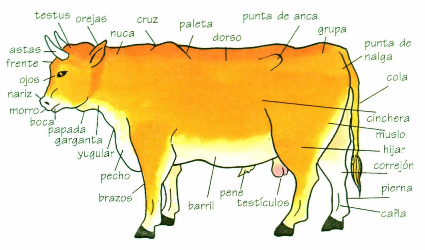
\includegraphics[scale=0.9]{img/dibujito1.png}
 \end{center}
 \caption{Partes físicas de un bovino. Tomada de \cite{librito1}}
\end{figure}

%%% Tek: faltan lsa refs para las figs

\subsubsection{Clasificación vacuna por aptitud productiva}
\begin{itemize}
\item \textbf{Lechero:} (Cabe resaltar que un requerimiento o propiedad fisonómica básica es que posean ubre, esto quiere decir solo las hembras pueden hacer parte de esta aptitud productiva). Poseen formación triangular, cuentan con cuerpo y extremidades largas y delgadas con poca voluminosidad cárnica
\begin{figure}[H]
 \begin{center}
 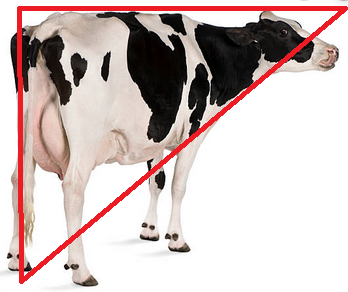
\includegraphics[scale=0.9]{img/dibujito2.png}
 \end{center}
 \caption{Aptitud lechera. Tomada de \cite{googlepics}. }
\end{figure}
\item \textbf{Carne:} Poseen una contextura rectangular. Además de poseer un cuerpo ancho con sus extremidades bien dotadas de carne.
\begin{figure}[H]
 \begin{center}
 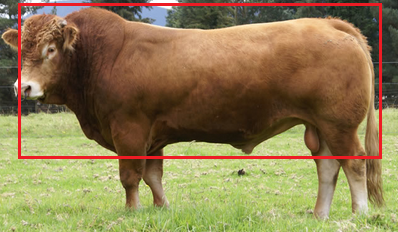
\includegraphics[scale=0.9]{img/dibujito3.png}
 \end{center}
 \caption{Aptitud de tipo carne. Tomada de \cite{googlepics}. }
\end{figure}
\item \textbf{Doble propósito:} Cuentan con propiedades mixtas de los 2 tipos ya mencionados, por lo que tanto su contextura, como volumen cárnico, ubre y extremidades son medianas. Este tipo de animales poseen una mayor facilidad en la adaptación del clima, alimentación y manejo. 
\begin{figure}[H]
 \begin{center}
 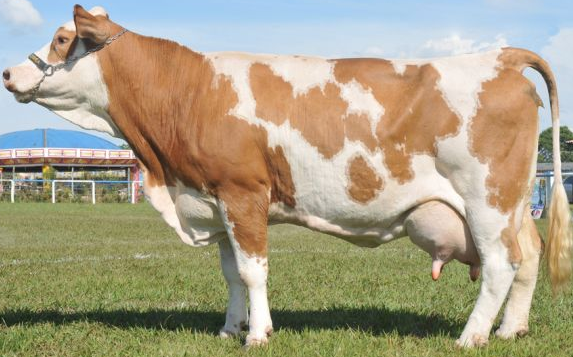
\includegraphics[scale=0.8]{img/dibujito4.png}
 \end{center}
 \caption{Aptitud de doble propósito.  Tomada de \cite{googlepics}. \label{}}
\end{figure}
\end{itemize}

% A modo general y para el desarrollo de este trabajo desde este punto en adelante, se decide describir más a fondo el ganado vacuno y enfocarse en describir de manera más profunda las ganaderías de la carne y la leche.\\


En el Cauca, aunque se cuente con abundantes hectáreas de diferentes fertilidades y condiciones térmicas apropiadas para el cultivo y desarrollo de la ganadería, se presentan muchas falencias en materia tecnológica y económica, en donde los movimientos migratorios de campesinos desplazados y los efectos colaterales del conflicto armado que se ha presentado en el país, son las principales causas de estas falencias. Sin embargo, el emprendimiento de los pequeños y medianos productores da paso a nuevas oportunidades de intervención por parte de la ingeniería electrónica y el manejo aplicativo de nuevas tecnologías que permitan tener un contacto más cercano con la población campesina.\\



Lo anterior se diseña y se plantea acorde con el manual de Buenas Prácticas de Ganadería  (BPG) y con las legislaciones pertinentes al manejo de alimentos para el consumo humano establecidas por la ley colombiana mencionados en la sección \ref{leyes}.

%%%%%%%%%%%%%%%%%%

\section{Sistemas de explotación del ganado vacuno}

Indiferentemente de su aptitud productiva, el ganado vacuno debe situarse en una infraestructura o ambiente apropiado para su desarrollo. Sin embargo, por  cuestiones geográficas, geológicas y/o climatológicas, los animales son criados mediante métodos de explotación como el estabulado, semiestabulado y el silvopastoril:\\

\begin{figure}[H]
 \begin{center}
 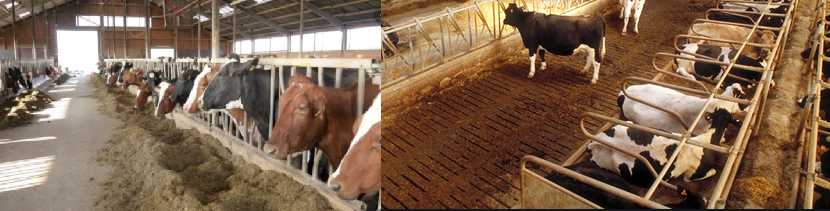
\includegraphics[scale=0.8]{img/estabulado.png}
 \end{center}
 \caption{Sistema de explotación estabulada. Tomada de \cite{googlepics}. \label{estabulpng}}
\end{figure}

El sistema ``estabulado'' (Ver figura \ref{estabulpng}) es una forma de crianza de ganado en la cual los animales pasan la mayor parte del tiempo en establos donde realizan sus actividades diarias. En estos establos se recrea la vida del ganado con la diferencia que el mismo se encuentra protegido bajo techo sin tener exposición directa al sol y a las condiciones medio ambientales. En este sistema se pretende una mayor producción y mejor calidad de la carne en el menor tiempo posible \cite{defestabulacion}.\\

 Por su parte el sistema ``silvopastoril' (ver Figura \ref{silvopng})' es una forma de cultivo agropecuario que involucra la presencia de árboles interactuando con gramíneas y los animales sometidos a un manejo determinado para incrementar la productividad y el beneficio neto de la explotación a mediano y corto plazo \cite{defsilvopas}.

\begin{figure}[H]
 \begin{center}
 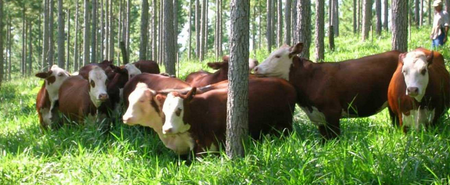
\includegraphics[scale=0.9]{img/silvopastoril.png}
 \end{center}
 \caption{Sistema de explotación silvopastoril. Tomada de \cite{contextoganadero}. \label{silvopng}}
\end{figure}

Finalmente, en el sistema semiestabulado se combinan los 2 sistemas mencionados. En este sistema mixto, los animales ingieren sus raciones de alimento principal en áreas extensas de pastos y forrajes vegetales, mientras que el cuidado y el suministro especializado de vitaminas y proteínas se realiza bajo techo.
%\begin{figure}[H]
% \begin{center}
% \includegraphics[scale=0.6]{img/tiposdosif.png}
% \end{center}
% \caption{Sistema de explotación por estabulación.  \label{estabulpng}}
%\end{figure}
%\begin{figure}[H]
% \begin{center}
% \includegraphics[scale=0.6]{img/tiposdosif.png}
% \end{center}
% \caption{Sistema de explotación silvopastoril. \label{silvopng}}
%\end{figure}
\subsection{Ciclo productivo de la leche}

% 2/10/2022 Cambiar la iamgen por una que tenga que ver con leche y luego descomentar el begin figure 
% \begin{figure}[H]
% \begin{center}
% 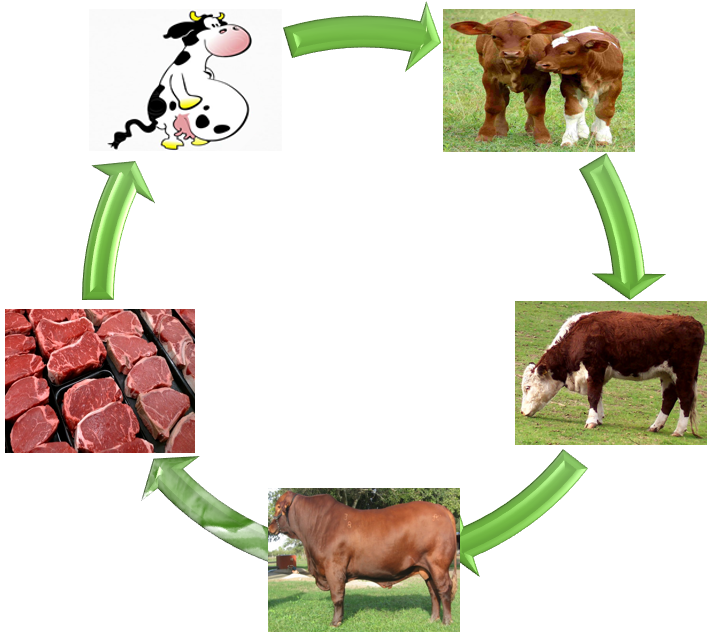
\includegraphics[scale=0.45]{img/ganadcarne.png}
% \end{center}
% \caption{Ciclo productivo en la ganadería de ordeño. \label{ganadcarnepng}}
% \end{figure}

% (Ver Figura \ref{ganadcarnepng}) 
 
El ciclo productivo de la leche de un ganado destinado para tal fin consta de 3 etapas principales que abarcan desde la gestación de la cría y maxima producción de leche, seguido de un periodo de declive y persistencia de producción y finalizando con el periodo de secado en donde se da descanso a la vaca para que se regenere el tejido glandular productor de leche para la siguiente lactancia \cite{mahecha}.\\

Estas etapas son brevemente descritas a continuación:


% \begin{itemize}
    \subsubsection{Etapa de crianza:} Es la etapa de producción temprana en donde el animal (generalmente crías hembras denominadas terneras) son alimentadas y criadas hasta alcanzar 2 años de edad.
	\begin{itemize}
% 		\item En esta etapa se requiere de grandes extensiones de tierra para producir crías
		\item No requiere de estaciones climatológicas específicas y se puede dar en todo el año (Esta característica varía dependiendo de la ubicación geográfica y las exposiciones climatológicas).
		\item Los elementos principales en la dieta de estas criaturas son los nutrientes provenientes del Calostro, la leche materna, forraje y vitaminas.\\
	\end{itemize} 
	\subsubsection{Etapa de gestación y ordeño:} Es la etapa inmediatamente siguiente a la etapa de crianza, en donde la novilla esta desarrollada y en la capacidad de ser inseminada para iniciar su producción de leche.
	\begin{itemize}
% 		\item En esta etapa se estima que el peso del animal puede alcanzar un mínimo de 230[kg] de peso en adelante.
% 		\item Es considerada como la etapa más rentable debido a las  pocas exigencias en materia de calidad alimenticia. 
		\item El objetivo de esta etapa es que la novilla produzca leche mientras que se da la gestación del novillo dentro de ella.
		\item El alimento se basa en pasturas de calidad, provenientes de las extensiones de tierra donde comen las reses y se crían.
		\item El animal gana mayor peso debido a su etapa de crecimiento, por lo que entre mejor sea su alimentación se obtendrán mejores resultados.
		\item Es de vital importancia que el animal se encuentre en la capacidad de  alimentarse \texit{Ad Libitum}, es decir a placer y a voluntad.
		\item En esta etapa, la novilla es denominada primípara, pues se encuentra abarcando el tiempo de gestación de su primera cría.\\
	\end{itemize} 
	\subsubsection{Etapa seca o de secado:} Es la etapa final que abarca los últimos 2 meses de gestación previos al parto en donde se da paso a la regeneración de tejidos glandulares que producen leche y a la curación de las glándulas mamarías para reducir el riesgo de mastitis. En sus características principales se pueden mencionar:
	\begin{itemize}
		\item Aún cuando la novilla primípara esta en capacidad de producir leche, no se debe recurrir al ordeño hasta que no se realice el parto.
	\end{itemize}
% \end{itemize} 

\subsubsection{Razas}

Debido a la gran variedad de especies, condiciones ambientales, y al proceso evolutivo del ganado, históricamente se ha podido clasificar y seleccionar las razas más representativas para este tipo de explotación ganadera. Más precisamente se puede hacer mención de las siguientes:
\begin{multicols}{2}
    \begin{center}
        \begin{itemize}
        \item Simmental
        \item Holstein
        \item Jersey
        \item Normando
        \end{itemize}
    \end{center}
\end{multicols}

Éstas son seleccionadas principalmente por la contextura voluminosa pero factores como la calidad de la leche pueden sobrepasar los criterios cuantitativos. A continuación se muestran algunos ejemplares de estas razas:

\begin{figure}[H]
 \begin{center}
 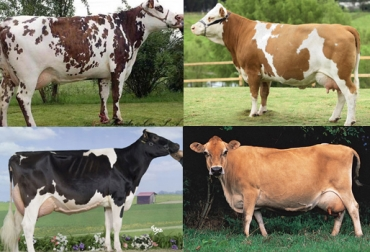
\includegraphics[scale=1]{img/razaslecheras.png}
% \end{center}
 \caption{En la primer fila de izquierda a derecha se observan ejemplares de las razas Normando, Simmental; seguido de las razas Holstein y Jersey en la fila inferior. Tomada de \cite{contextoganadero} \label{cuadrorazaspng}}
  \end{center}
\end{figure}

\subsection{Ciclo productivo de la carne}

\begin{figure}[H]
\begin{center}
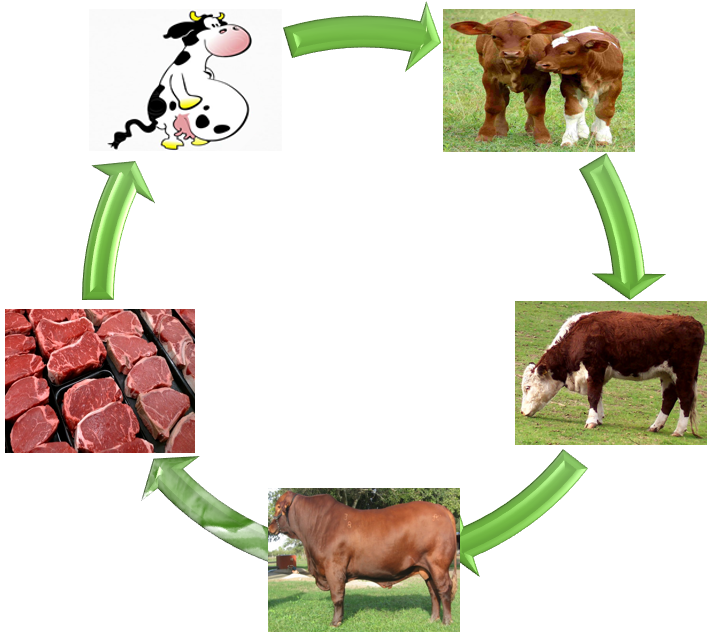
\includegraphics[scale=0.55]{img/ganadcarne.png}
\end{center}
\caption{Ciclo productivo en la ganadería de la carne.  Tomada de \cite{contextoganadero}. \label{ganadcarnepng}}
\end{figure}

 
El ciclo productivo de la carne (Ver Figura \ref{ganadcarnepng})  de un ganado destinado para tal fin consta de 3 etapas principales que abarcan desde el nacimiento de la cría, su desarrollo y crecimiento y finalizando con su comercialización en el momento en que alcanza las condiciones apropiadas para ser transformado en carne para consumo humano \cite{mahecha}. Estas etapas son brevemente descritas a continuación:


%y finalizando en el momento en que alacanza las condiciones apropiadas para ser transformado en carne para consumo humano \cite{mahecha}. Estas etapas son brevemente descritas a continuación:

\begin{itemize}
	\item \textbf{Ganadería de Cría:} Es la etapa de producción temprana en donde el animal (generalmente crías macho llamadas bovinos) es alimentado y criado desde su nacimiento hasta los primeros seis (6) meses de edad. 
	\begin{itemize}
		\item En esta etapa se requiere de grandes extensiones de tierra para producir crías
		\item No requiere de estaciones climatológicas específicas y se puede dar en todo el año.
		\item Los elementos principales en la dieta de estas criaturas son los nutrientes provenientes del Calostro y la leche materna.\\
	\end{itemize} 
	\item \textbf{Ganadería de Levante:} Es la etapa inmediatamente siguiente a la etapa de crianza, en donde el bovino se desarrollará entre los siete (7) y diez y ocho (18) meses de edad.
	\begin{itemize}
		\item En esta etapa se estima que el peso del animal puede alcanzar un mínimo de 230[kg] de peso en adelante.
		\item Es considerada como la etapa más rentable debido a las  pocas exigencias en materia de calidad alimenticia. 
		\item El objetivo de esta etapa es que el sujeto en cuestión alcance el peso deseado en el menor tiempo posible con el menor esfuerzo posible
		\item El alimento se basa en pasturas de calidad, provenientes de las extensiones de tierra donde comen las reses y se crían.
		\item El animal gana mayor peso debido a su etapa de crecimiento, por lo que entre mejor sea su alimentación se obtendrán mejores resultados.
		\item Es de vital importancia que el animal se encuentre en la capacidad de  alimentarse \texit{Ad Libitum}, es decir a placer y a voluntad.\\
	\end{itemize} 
	\item \textbf{Ganadería de engorde o Ceba:} Es la etapa final que abarca desde los 19 meses de edad hasta los 24 o 36 meses, dependiendo de su crecimiento  y otros factores como el interés del productor, la demanda del mercado, entre otras. En sus características principales se pueden mencionar:
	\begin{itemize}
		\item El límite se define por los intereses del productor, la demanda del mercado y en general por el peso ideal del animal que es aproximadamente mayor o igual a los 450[kg].
		\item Para la alimentación se requieren de buenas, grandes y controladas cantidades con el fin de mejorar la carne. Para esto se utilizan dietas que requieren pasturas y concentrados dietarios.
		\item Se debe monitorear la alimentación tomando registro en la ganancia de gramaje diaria de cada uno de los animales.
	\end{itemize}
\end{itemize} 

\subsubsection{Razas} Debido a la gran variedad de especies, condiciones ambientales, y al proceso evolutivo del ganado, históricamente se ha podido clasificar y seleccionar las razas más representativas para este tipo de explotación ganadera. Más precisamente se puede hacer mención de las siguientes:
\begin{multicols}{2}
\begin{center}
\begin{itemize}
\item Beefmaster
\item Charolais
\item Simmental
\item Angus
\item Brangus
\item Santa Gertrudis
\item Hereford
\item Limousin
\item Cebú
\item Belgina Blue
\end{itemize}
\end{center}
\end{multicols}

Éstas son seleccionadas principalmente por la contextura voluminosa pero factores como la calidad de la carne pueden sobrepasar los criterios cuantitativos. A continuación se muestran algunas de las razas más usadas para este propósito:

\begin{figure}[H]
 \begin{center}
 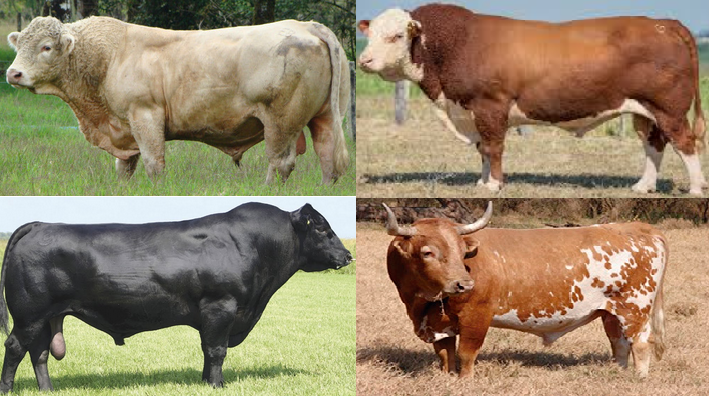
\includegraphics[scale=0.8]{img/cuadrorazas.png}
% \end{center}
 \caption{En la primer fila de izquierda a derecha se observan ejemplares de las razas Charolais, Hereford; seguido de las razas Angus y Criolla en la fila inferior.  Tomada de \cite{contextoganadero}. \label{cuadrorazaspng}}
  \end{center}
\end{figure}


\subsection{Alimentación y Componentes básicos de la dieta}
%\section{Marco de referencia}
% \subsubsection{Alimentación}
La alimentación de un cultivo de ganado requiere de una dieta o ración con diferentes componentes básicos o nutrientes que deben ser suministrados día a día de forma balanceada para lograr un crecimiento óptimo y que los animales puedan expresar su potencial genético \cite{recomendaciones}.\\

Los componentes principales que conforman la dieta alimenticia  del ganado son:
% 	\begin{itemize}
	

\subsubsection{Agua}
    Componente principal de la alimentación. Esta debe ser suministrada en cantidad y calidad para ser aprovechada por cada animal llegando a ocupar más del 50\% de la masa corporal de un ejemplar adulto y hasta un 90 \% de un recién nacido.
    	
	\begin{figure}[H]
	 \begin{center}
	 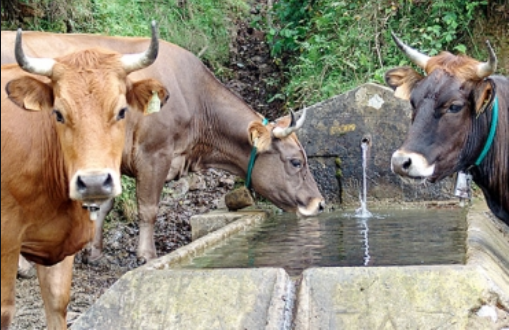
\includegraphics[scale=0.8]{img/agua.png}
	 \end{center}
	 \caption{Hidratación del ganado. Tomada de \cite{contextoganadero}.	\label{energeticospng}}
	\end{figure}
    	
\subsection{Energía}
Este componente se suministra mediante azúcares, almidones, celulosa, entre otros, los cuales aportan grandes cantidades de energía mas no de proteína, razón por la cual se deben suministrar de forma complementaria.
	\begin{figure}[H]
	 \begin{center}
	 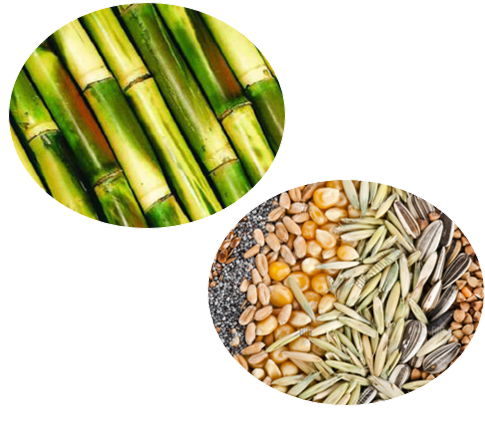
\includegraphics[scale=0.7]{img/melazacana.png}
	 \end{center}
	 \caption{Suplementos energéticos. 	\label{energeticospng}}
	\end{figure}
    
\subsection{Proteínas}
Estos nutrientes son fundamentales especialmente durante los periodos de sequía, por consiguiente, se optan por fuentes altas en proteína como leguminosas forrajeras, el Maní, Leucaena y el más común, los pastos de forraje verde. 
	\begin{figure}[H]
	 \begin{center}
	 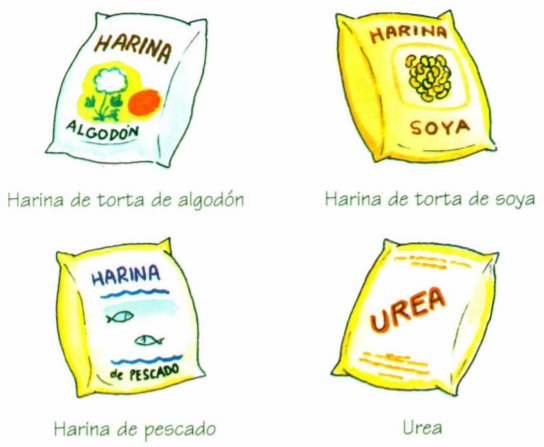
\includegraphics[scale=0.8]{img/proteina.png}
	 \end{center}
	 \caption{Suplementos proteínicos. Tomada de \cite{librito1}. \label{proteinaspng}}
	\end{figure}

\subsection{Minerales}
Son indispensables en la ganancia de peso de los novillos durante la etapa de Cría y Levante. Este complemento alimenticio debe estar siempre a la disposición para que el ganado pueda abastecer sus necesidades. Estos minerales se suelen proporcionar mediante mezclas de macrominerales y microminerales que se ofrecen de libre consumo al ganado.

\subsection{Vitaminas}
Suministradas en cantidades pequeñas aplicadas comúnmente en animales cuya alimentación se basa en forrajes secos,  o en animales enfermos convalecientes, desnutridos o durante épocas de sequía prolongada.
	\begin{figure}[H]
	 \begin{center}
	 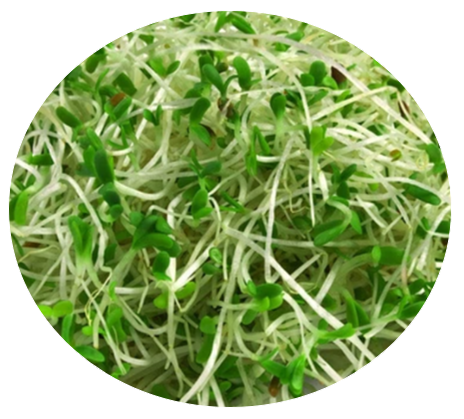
\includegraphics[scale=0.6]{img/leguminosas.png}
	 \end{center}
	 \caption{Forraje y leguminosas. Tomada de \cite{librito1}. \label{vitaminaspng}}
	\end{figure}

\subsection{Balance de raciones y dietas especializadas}
% \subsubsection{Balance de raciones y dietas especializadas}
    Estas dietas son suministradas por personal técnico calificado que prepara un dieta acorde a la cantidad de nutrientes de cada animal de forma particular e independiente, considerando su peso actual, su velocidad de crecimiento y estado fisiológico.

\subsection{Desperdicios}

\section{Leyes y Normatividad}  \label{leyes}
Requerida para que el avance ganadero se realice de manera coordinada o estandarizada basada en las buenas prácticas ganaderas en pro de mejorar la productividad y ayudarla a alcanzar niveles de ganadería bovina del mundo \cite{invima}, \cite{leylacteos}, \cite{minsaludleche}. 
\begin{itemize}
	\item \textbf{Resolución 2310 de 1986:} Reglamentación parcial en el titulo V de la ley 09 de 1979 que se refiere al procesamiento, composición, requisitos, transporte, y comercialización de los Derivados Lácteos.
	\item \textbf{Resolución 11961 de 1989:} Reglamentación parcial a la resolución 2310 de 1986 que se refiere a lo relacionado con las clases de leche fermentada.
	\item \textbf{Decreto 0616 de 2006:} Reglamento técnico sobre los requisitos que debe cumplir la leche para el consumo humano que se obtenga, procese, envase, transporte, comercialice, expenda, importe o exporte en el país.
	\item \textbf{Resolución 0012 de 2007:} Por la cual se establece el sistema de pago de la leche cruda al productor, diseñado por la Unidad de Seguimiento de Precios.
	\item \textbf{Decreto 1500 de 2007:} Reglamento técnico a través del cual se crea el Sistema Oficial de Inspección, Vigilancia y Control de la Carne y otros productos comestibles y derivados cárnicos destinados para el consumo humano.
	\item \textbf{Decreto 072 de 2007:} Por el cual se establece el manual de buenas prácticas de manejo para la producción de ganado bovino.
	\item \textbf{Decreto 2905 de 2007:} Por el cual se establece el reglamento técnico sobre los requisitos sanitarios y de inocuidad de la carne y productos cárnicos comestibles de las especies bovina y bufalina destinados para el consumo humano.
	\item \textbf{Decreto 18119 de 2007:} Por el cual se reglamenta los requisitos del plan gradual de cumplimiento para  las plantas de beneficio y desposte de bovino y bufalinos.
	\item \textbf{Decreto 2278 de 1982:} Reglamentación parcial en el titulo V de la ley 09 de 1979 que se refiere al sacrificio de animales de abasto público o para consumo humano y el procesamiento, transporte y comercialización de su carne.

\end{itemize}

% \section{Conceptos adicionales}
% \item \textbf{Jáquima:} Es un freno, cabestro o cabezada usado en la ganadería principalmente equina, para identificar, amansar o manipular al animal \cite{jaquima}.

% %%%%%Productos y resultados que se entregarán cuando finalice el proyecto (1/2 página). 
